\newcommand{\nauticleversion}{1.0.170221}
\newcommand{\installer}{install-\nauticleversion{}.sh}
\newcommand{\uninstaller}{uninstall-\nauticleversion{}.sh}
\newcommand{\execname}{\textbf{nausolve}}

\documentclass[a4paper,12pt,openany]{book}
% \documentclass[a4paper,12pt,openany]{paper}
\usepackage{courier}
\usepackage[utf8]{inputenc}
\usepackage[T1]{fontenc}
\usepackage[english]{babel} % If you write in English
\usepackage{a4wide}
\usepackage{graphicx}
\graphicspath{{images/}}
\usepackage{subfig}
\usepackage{tikz}
\usetikzlibrary{shapes,arrows}
\usepackage{pgfplots}
\pgfplotsset{compat=newest}
\pgfplotsset{plot coordinates/math parser=false}
\newlength\figureheight
\newlength\figurewidth
\pgfkeys{/pgf/number format/.cd,
set decimal separator={,\!},
1000 sep={\,},
}
\usepackage{ifthen}
\usepackage{ifpdf}
\ifpdf
\usepackage[pdftex]{hyperref}
\else
\usepackage{hyperref}
\fi
\usepackage{color}
\usepackage{xcolor}
\usepackage{listings}
\usepackage{indentfirst}
\lstset{
  basicstyle=\ttfamily,
  showstringspaces=false,
  commentstyle=\color{red},
  keywordstyle=\color{blue},
  escapeinside={(*@}{@*)},
}
\usepackage[many]{tcolorbox}
\usepackage{lipsum}
\newtcbtheorem[]{example}{}{
  breakable,
  enhanced,
  colback=blue!5,
  colframe=blue!35!black,
  fonttitle=\bfseries}{x}

\hypersetup{%
colorlinks=true,
linkcolor=black,
citecolor=black,
urlcolor=black}
\definecolor{nauticlegreen}{RGB}{153, 204, 0}
\definecolor{nauticlegreen_dark}{RGB}{110, 150, 0}

\renewcommand{\baselinestretch}{1.05}
\renewcommand\thesection{\arabic{section}}
\usepackage{fancyhdr}
\pagestyle{fancy}

\usepackage{amsthm}
\usepackage{amssymb,amsmath,bbm}
\usepackage{array}
\usepackage{bm}
\usepackage{multirow}
\usepackage[footnote]{acronym}
\usepackage{algorithm}
\usepackage[noend]{algpseudocode}

\newcommand*{\SET}[1]  {\ensuremath{\mathbf{#1}}}
\newcommand*{\VEC}[1]  {\ensuremath{\boldsymbol{#1}}}
\newcommand*{\FAM}[1]  {\ensuremath{\boldsymbol{#1}}}
\newcommand*{\MAT}[1]  {\ensuremath{\boldsymbol{#1}}}
\newcommand*{\OP}[1]  {\ensuremath{\mathrm{#1}}}
\newcommand*{\NORM}[1]  {\ensuremath{\left\|#1\right\|}}
\newcommand*{\DPR}[2]  {\ensuremath{\left \langle #1,#2 \right \rangle}}
\newcommand*{\calbf}[1]  {\ensuremath{\boldsymbol{\mathcal{#1}}}}
\newcommand*{\shift}[1]  {\ensuremath{\boldsymbol{#1}}}

\newcommand{\eqdef}{\stackrel{\mathrm{def}}{=}}
\newcommand{\argmax}{\operatornamewithlimits{argmax}}
\newcommand{\argmin}{\operatornamewithlimits{argmin}}
\newcommand{\ud}{\, \mathrm{d}}
\newcommand{\vect}{\text{Vect}}
\newcommand{\sinc}{\ensuremath{\mathrm{sinc}}}
\newcommand{\esp}{\ensuremath{\mathbb{E}}}
\newcommand{\hilbert}{\ensuremath{\mathcal{H}}}
\newcommand{\fourier}{\ensuremath{\mathcal{F}}}
\newcommand{\sgn}{\text{sgn}}
\newcommand{\intTT}{\int_{-T}^{T}}
\newcommand{\intT}{\int_{-\frac{T}{2}}^{\frac{T}{2}}}
\newcommand{\intinf}{\int_{-\infty}^{+\infty}}
\newcommand{\Sh}{\ensuremath{\boldsymbol{S}}}
\newcommand{\C}{\SET{C}}
\newcommand{\R}{\SET{R}}
\newcommand{\Z}{\SET{Z}}
\newcommand{\N}{\SET{N}}
\newcommand{\K}{\SET{K}}
\newcommand{\reel}{\mathcal{R}}
\newcommand{\imag}{\mathcal{I}}
\newcommand{\cmnr}{c_{m,n}^\reel}
\newcommand{\cmni}{c_{m,n}^\imag}
\newcommand{\cnr}{c_{n}^\reel}
\newcommand{\cni}{c_{n}^\imag}
\newcommand{\tproto}{g}
\newcommand{\rproto}{\check{g}}
\newcommand{\LR}{\mathcal{L}_2(\SET{R})}
\newcommand{\LZ}{\ell_2(\SET{Z})}
\newcommand{\LZI}[1]{\ell_2(\SET{#1})}
\newcommand{\LZZ}{\ell_2(\SET{Z}^2)}
\newcommand{\diag}{\operatorname{diag}}
\newcommand{\noise}{z}
\newcommand{\Noise}{Z}
\newcommand{\filtnoise}{\zeta}
\newcommand{\tp}{g}
\newcommand{\rp}{\check{g}}
\newcommand{\TP}{G}
\newcommand{\RP}{\check{G}}
\newcommand{\dmin}{d_{\mathrm{min}}}
\newcommand{\Dmin}{D_{\mathrm{min}}}
\newcommand{\Image}{\ensuremath{\text{Im}}}
\newcommand{\Span}{\ensuremath{\text{Span}}}
\newcommand{\equref}[1]{(\ref{#1})}
\newcommand{\myhref}[3][nauticlegreen_dark]{\href{#2}{\color{#1}{#3}}}%
\newcommand{\norm}[1]{\left\lVert#1\right\rVert}
\newcommand{\puretext}[1]{\quad\textrm{#1}\quad}
\newcommand{\myparagraph}[1]{\paragraph{#1}\mbox{}\\}
\usepackage{mathtools}
\DeclarePairedDelimiter\floor{\lfloor}{\rfloor}

\usepackage{tabularx,ragged2e,booktabs,caption}
\newcolumntype{C}[1]{>{\Centering}m{#1}}
\renewcommand\tabularxcolumn[1]{C{#1}}


\newtheoremstyle{break}
  {11pt}{11pt}%
  {\itshape}{}%
  {\bfseries}{}%
  {\newline}{}%
\theoremstyle{break}

%\theoremstyle{definition}
\newtheorem{definition}{Définition}[chapter]

%\theoremstyle{definition}
\newtheorem{theoreme}{Théorème}[chapter]

%\theoremstyle{remark}
\newtheorem{remarque}{Remarque}[chapter]

%\theoremstyle{plain}
\newtheorem{propriete}{Propriété}[chapter]
\newtheorem{exemple}{Exemple}[chapter]

\parskip=5pt
%\sloppy

\setcounter{secnumdepth}{5}

\begin{document}
%%%%%%%%%%%%%%%%%%
%%% Title page %%%
%%%%%%%%%%%%%%%%%%
\frontmatter
\begin{titlepage}
\begin{center}
\vspace{5cm}

\includegraphics[width=0.6\textwidth]{nauticle_logo.pdf}\\[0.5cm]
{\large A particle based meshless numerical computational environment}\\ [5cm]
% Title
{ \huge \bfseries User Guide for Nauticle \\[0.2cm] }
\color{nauticlegreen}
\rule{\linewidth}{1.5mm} \\[0.5cm]
\color{black}
{\large Nauticle version: \nauticleversion{} \\ \today}
% Bottom of the page
\vfill
% Author and supervisor
\noindent
\begin{minipage}{1\textwidth}
  \begin{flushright} \large
    \emph{Author :}\\
    Balázs TÓTH \\
    Toth.Balazs@epito.bme.hu
  \end{flushright}
\end{minipage}
\end{center}
\end{titlepage}
\clearpage\mbox{}\clearpage
\chapter{Abstract}
This manuscript provides a detailed introduction of the Nauticle solver. It contains an installation and calculation guide beside the presentation of the Nauticle interface. The latter allows any user to embed the solver with new particle-based schemes as interactions - or even arbitrary models considered as black boxes - without the deep insight to the core of the solver.

\tableofcontents
\newpage
\mainmatter

\raggedbottom
\section{Introduction}
Due to their attractive properties, particle-based numerical methods enjoy increasing attention in many fields of engineering applications. In contrast with mesh-based methods  like finite element method, particle shemes have more flexible and adaptable spatial discretisation of the computational domain of any shape, especially in case of large deformations involving topology changes even with domain splitting [TODO].
From the implementation point of view, most of the common features of particle-based numerical schemes are fundamentally different from mesh-based methods. Some of these differences are the lack of internodal structure (mesh), persistent changing of nodal connectivity, overlapping spatial covering of computational domain.

During the past decades several meshless numerical solver like [TODO], successfully proved the reason of existence of particle methods. These tools have solved problems of free surface flows, fluid-solid interactions, crack growth and propagation in solid domain, underwater explosions, in which areas mesh-based methods usually suffer from serious bottlenecks. Furthermore, the naturally large requirement of computational performance can be compensated by the efficient massive parallelisation of computations on multicore CPU and GPU devices. However, most of these simulation tools are designed to employ on a certain particle scheme, moreover, the governing equations of the physical model is usually burried in the code. The lack of generality from both the physical model and the computational scheme point of view, results in a robust but rigid numerical engine with limited range of applications. % ok 

To leap towards a more general formulation of computations, one needs to distinguish two aspects of generality. The first one is that it is inevitable to emerge the governing equations from the depth of the solver core to the user's level. Obviously, it requires a fundamentally different realisation of the solver but ensures higher flexibility at the same time. The second aspect is that the governing equations should be interpreted and discretised according to a suitable numerical method, consequently several different methods need to be implemented in the same environment. Using a proper formulation for the interface between the solver core, the different numerical schemes and the user-defined equations it turns out that a truly flexible meshless simulation tool can be established. Note that the existence of multipurpose schemes in a single environment significantly facilitates  not only the flexible modelling of almost arbitrary problems but the efficient simulation of coupled problems as well.

Nauticle is a general-purpose open-source C++ scientific numerical environment and solver for the application and implementation of particle methods. The goal of the library is to  establish a particle-based numerical solver that can solve user-defined system of algebraic and differential equtions over a set of spatially distributed particles in one, two, or three dimensions with the most suitable numerical particle-schemes. Solutions can be governed by priori implemented schemes like SPH, DEM, etc. 

The user-guide is organised as follows: TODO

\section{Methodology}
\subsection{Particle methods}
Several classification of particle methods exist based on different mathematical or physical aspects. From mathematical point of view we can distinguish methods that are operating on the strong form of Partial Differential Equations (PDE's) from those that are solving the weak form of PDE's. Another classification is possible based on the physical characteristics of the domain to be modeled. On the one hand, there are continuum domains such as fluids or solids, where the element of discretisation should represent a more or less intuitively delimited macroscopic portion of continuum phase, while on the other hand, there are granular phases, like sand or molecules, where each element is assigned to a physically existing individual material parcel or molecule. Here we focus on the concept of the latter, the physical classification.
\subsubsection{Continuum methods}
This subsection contains some of the fundamental considerations of continuum particle methods with the definitions provided by [TODO]. \\

\textbf{The $C^k$ spaces}: Let $\Omega$ be a bounded domain in $\R^d$ with piecewise continuous boundary $\partial\Omega$. We let $C^0(\Omega)$ denote the space of all continuous functions on $\overline{\Omega}$ with the norm
\begin{equation}
\norm{u}_{C^0(\Omega)}=max_{x\in\overline{\Omega}}|u(x)|,
\end{equation}
where $u(x)\in\R$. We denote
\begin{equation}
C^k(\Omega):=\{v\in C^0\vert\norm{v}_{C^k (\Omega)}<\infty\},
\end{equation}
where
\begin{equation}
\norm{v}_{C^k (\Omega)}:=\sum_{0<j<k}\sum_{m_{1j}+m_{2j}+...m_{dj}=j}\norm{\frac{\partial^j u}{\partial x^{m_{1j}}_{\partial x_1}\partial x^{m_{2j}}_{\partial x_2}...\partial x^{m_{dj}}_{\partial x_d}}}_{C^0(\Omega)}
\end{equation}
We also denote $C^0(\Omega)$ as the space of all continuous functions on $\Omega$ that also vanish at $\partial\Omega$

\textbf{Partition of Unity}: Let $\Omega \subset \R^d(d=1,2,3)$ be and open bounded domain. Let $\Omega_1$, $\Omega_2$, ... $\Omega_{NP}$ be a family of open sets in $\R^d$, and \\
1. The family of an open set ${\Omega}_{I\in\Lambda}$ generates a covering for domain $\Omega$,
\begin{equation}
\Omega\subset\bigcup\limits_{I\in \Lambda} \Omega_I
\end{equation}
2. There exists a family of functions, $\phi_I\in C_0^s(\R^d)$, $s\geq 0$, and $supp\{\phi_I\}\subset \overline{\Omega}_I$

\noindent
3.
\begin{equation}
0\leq\phi_I\leq 1 \quad \forall x \in \Omega_I
\end{equation}
4. The summation
\begin{equation}
\phi_1(\textbf{x})+\phi_2(\textbf{x})+\phi_3(\textbf{x})+\cdots+\phi_{NP}(\textbf{x})=1, \quad \forall \textbf{x}\in\Omega
\end{equation}
the family of generating function, or interpolation basis, ${\phi_I}_{I\in\Lambda}$ is called a partition of unity subordinate to the open cover $\{\Omega_I\}_{I\in \Lambda}$.

A peculiar consequence of the partition of unity is that the open supports can form an overlapping covering of the computational domain. The essential principle of particle methods is founded on the concept of partition of unity (meshfree interpolation), which is constructed using $\phi$ mollifier functions with specific properties:
\begin{flalign}
\begin{split}
&1.\quad \phi\in C^k(\Omega) \quad \textrm{where} \quad k>1, \\
&2.\quad supp\{\phi\}=B_1, \\
&3.\quad \phi(\textbf{x})>0 \quad \textrm{for} \norm{x}<1, \\
&4.\quad \int_{B_1}\phi(\textbf{x})d\Omega=1,
\end{split}
\end{flalign}
where
\begin{align}
B_{\rho}(\overline{\textbf{x}})=\{\textbf{x}|\norm{\textbf{x}-\overline{\textbf{x}}}\leq\rho,\textbf{x}\in \R^d\}
\end{align}
denotes a closed spherical ball shaped domain of influence with radius $\rho$ around $\overline{\textbf{x}}$. \\

Some of the continuum methods are Smoothed Particle Hydrodynamics (SPH), which is a special collocation scheme for solving the strong form of PDE's, Element Free Galerkin method (EFG), Meshless Local Petrov Galerkin (MLPG), Reproducing Kernel Particle Method (RKPM), which are operating with weak form PDE's.
\subsubsection{Discrete methods}
In contrast with the representation of continuum domains, discrete methods do not apply meshfree interpolation techniques. Instead, the interactions (e.g. collisions) of macroscopic or molecular elements are directly calculated using physics-based models. Obviously, in the case of these methods, no spatial discretisation is required, due to the layout provided by the physical domain.

These methods are the Discrete Element Method (DEM), Molecular Dynamics (MD), and we can mention here the simulations of self-gravitating multibody problems. Furthermore, the simulations of crowd, traffic, cloud of cooperating drones, or almost any problem, in which the state of individual objects depend on each other and governed by specific interaction-laws.

\subsection{Methods implemented in Nauticle} \label{sec:implemented}
Nauticle itself can be considered as an empty frame, until at least one numerical method is implemented and connected through its interface (see [TODO]). This section provides a brief introduction of three widespread particle methods, that are already implemented in Nauticle. The author encourages you to read the referred publications for more detailed and exhausting explanations in these topics.




\subsubsection{N-body dynamics}
The investigation of the dynamics of celestial objects with gravitational interaction has been motivated by the desire to calculate and predict the motion of the planets in the Solar system for arbitrary past or future times. The physical problem to solve in such a problem is often referred as the so-called N-body problem.
\myparagraph{Equation of motion}
In the multibody system the motion of a single object is governed by the
\begin{flalign} \label{DEM_tangential_force}
&\frac{d^2r_i}{dt^2}=\gamma\sum_j^N{\frac{m_im_j}{(r_i-r_j)^2}n},
\end{flalign}
where $\gamma$ is the gravitational constant, $m_i$ is the mass of object $i$, $N$ is the number of objects in the system, and again, $n=(r_i-r_j)/|r_i-r_j|$ is the normalised direction vector between the objects $i$ and $j$. Considering the planets as rotationally invariant spherical objects, their angular motion does not influence the translational motions. This model has $N^2$ computational complexity.




\subsubsection{Smoothed Particle Hydrodynamics}
In the late 1970's the first papers on Smoothed Particle Hydrodynamics (SPH) published by R.A. Gingold and J.J. Monaghan [TODO] and independently by B. Lucy [TODO]. One of the motivations to construct SPH was the necessity of numerical methods dealing with boundaryless problems. Initially SPH was applied in astrophysical simulations, later, in the  early 1990's the first applications to fluid and solid mechanics problems appeared. During  the past two decades increasing attention is focused on SPH in both scientific and industrial areas, and the most significant progress of the development is done in the past fifteen years.\\
SPH is a fully meshless collocation scheme representing continuum fields with spatially distributed set of particles (meshless interpolation). The basic idea of SPH is the generalised interpolation
\begin{flalign} \label{convolution_delta}
  A(r)=\int_{\Omega}{A(r')\delta(r-r')dV},
\end{flalign}
where $A(r)$ is an arbitrary function, $\delta$ is the Dirac-function, and $\Omega$ is an opened or closed spatial domain. The convolution \equref{convolution_delta} is directly not applicable in numerical models due to two reasons. On the one hand, the Dirac-function is  neither continuous, nor finite. On the other hand, the intergration can be performed on analytic functions only.
The first step should be the application of a mathematically more favourable smoothing kernel or  mollifier function $W(r-r',\sigma)$ instead of the Dirac-function:
\begin{flalign} \label{convolution_kernel}
  A(r)=\int_{\Omega}{A(r')W(r-r')dV}.
\end{flalign}
The kernel function $W(r-r',\sigma)$ has infinite or finite influence radius, with a $\sigma$ parameter controlling the width of the function. Here it is assumed that $W(r-r',\sigma)$ has finite radius denoted by $\Delta=n\sigma$, with $n\in\N$. The choice of the smoothing kernel function is not arbitrary. The most important properties of any smoothing kernel are (recalling the properties of the mollifier functions in partition of unity):
\begin{flalign} \label{kernel_properties}
\begin{split}
&1.\quad W(r-r',\sigma)\in C^k(\Omega) \puretext{where} k>1, \\
&2.\quad supp(W(r-r',\sigma))=B', \\
&3.\quad W(r-r',\sigma)>0 \puretext{if} \norm{r}<\Delta, \\
&4.\quad \int_{\Omega}{W(r-r',\sigma)dV}=1, \\
&5.\quad \lim_{\sigma\to 0}W(r-r',\sigma)=\delta(r-r').
\end{split}
\end{flalign}
Here $B'$ is a spherical volume around $r$ with a radius of $\Delta$. \\
The discretisation of \equref{convolution_kernel} to a cloud of particles is written as
\begin{flalign} \label{discrete_convolution}
  \langle A(r_i)\rangle=\sum_{j}{A(r_j)W(r_i-r_j)\frac{m_j}{\rho_j}},
\end{flalign}
where $m_j$ and $\rho_j$ are the particle mass and density values of particle $j$ respectively. \\
The construction of first order SPH-differential operators can be introduced by applying \equref{convolution_kernel} to the derivative of $A(r)$. Using the divergence theorem of Gauss-Ostrogradsky, the second condition in \equref{kernel_properties}, and assuming that the sampling of the spherical domain $\Omega$ is sufficiently uniform, the differential operator can be replaced to the smoothing kernel function:
\begin{flalign} \label{continuum_diffop}
\begin{split}
  \nabla A(r)=\int_{\Omega}{(\nabla A(r'))W(r-r')dV} = \\
  \int_{\Omega}{\nabla \big[A(r')W(r-r')\big]dV}-\int_{\Omega}{A(r')\nabla W(r-r')dV}=\\
  \int_{\partial\Omega}{A(r')W(r-r')dS}-\int_{\Omega}{A(r')\nabla W(r-r')dV}=\\
  -\int_{\Omega}{A(r')\nabla W(r-r')dV}.
\end{split}
\end{flalign}
The discretised form of \equref{continuum_diffop} is as follows: 
\begin{flalign} \label{naive_diffop}
  \langle \nabla A(r_i)\rangle=\sum_{j}{A(r_j)\nabla W(r_i-r_j)\frac{m_j}{\rho_j}}.
\end{flalign}
Since the straightforward (or naive) differential operator \equref{naive_diffop} suffers from the lack of $0^{th}$ order consitency when the particle layout is not perfectly uniform, several attempts made to increase accuracy. The different formulas of differential operators form a trade-off between consistency and conservation properties, and the choice of a suitable operator is usually based on physical considerations of a specific problem.
Two of the most frequently applied first order SPH differential operators are 
\begin{flalign} \label{corrected_diffop1}
  &1.\quad\langle \nabla A(r_i)\rangle=\sum_{j}{\Bigg(\rho_j^k \frac{A(r_i)}{\rho_i^k}+\rho_i^k \frac{A(r_j)}{\rho_j^k}\Bigg)\nabla W(r_i-r_j)\frac{m_j}{\rho_j}}, \\
  &2.\quad\langle \nabla A(r_i)\rangle=\sum_{j}{\Bigg(\rho_i^k \frac{A(r_i)}{\rho_j^k}-\rho_j^k \frac{A(r_j)}{\rho_i^k}\Bigg)\nabla W(r_i-r_j)\frac{m_j}{\rho_j}},
  \label{corrected_diffop2}
\end{flalign}
where the power $k$ equals $0$ or $1$.\\
The construction of a second order differential operator requires some further considerations. Since the application of \equref{naive_diffop} to a second order  differentiation of $A(r)$
\begin{flalign}
  \langle \Delta A(r_i)\rangle=\sum_{j}{A(r_j)\Delta W(r_i-r_j)\frac{m_j}{\rho_j}}.
\end{flalign}
leads to a poor represention of the diffusion of quantity $A(r)$ [TODO], the invocation of the first order operators is more favourable. Considering \equref{corrected_diffop1} with $k=0$, the desired operator can be written as
\begin{flalign} \label{N2_second_order_diffop}
  \langle \Delta A(r_i)\rangle=\sum_{j}{\big(\langle\nabla A(r_i)\rangle+\langle\nabla A(r_j)\rangle\big)\nabla W(r_i-r_j)\frac{m_j}{\rho_j}}.
\end{flalign}
Although the \equref{N2_second_order_diffop} is mathematically correct, the implied nested interpolation has an undesirably high computational complexity. To evade this circumstance, the most prevailing practice is to approximate the embedded operators with Taylor-series expansions of $A(r)$ up to the first order around particles $i$ and $j$:
\begin{flalign} \label{Taylor_exp}
\begin{split}
A(r_j)=A(r_i)+\nabla A(r_i)(r_j-r_i), \\
A(r_i)=A(r_j)+\nabla A(r_j)(r_i-r_j).
\end{split}
\end{flalign}
After the expression of the derivatives of \equref{Taylor_exp} they can be inserted in \equref{N2_second_order_diffop}, to obtain the widespread second order SPH differential operator:
\begin{flalign} \label{secondorder_diffop1}
  \langle \Delta A(r_i)\rangle=\sum_{j}{2\big(A(r_i)-A(r_j)\big)\frac{r_j-r_i}{\vert r_j-r_i \vert^2}\nabla W(r_i-r_j)\frac{m_j}{\rho_j}},
\end{flalign}
which has a special variant
\begin{flalign} \label{secondorder_diffop2}
  \langle \nabla b\nabla A(r_i)\rangle=\sum_{j}{(b_i+b_j)\big(A(r_i)-A(r_j)\big)\frac{r_j-r_i}{\vert r_j-r_i \vert^2}\nabla W(r_i-r_j)\frac{m_j}{\rho_j}},
\end{flalign}
which is used to approximate the expression $\nabla b(r) \nabla A(r)$, with an arbitrary function $b$.
Employing the differential operators (\ref{corrected_diffop1}-\ref{secondorder_diffop2}), the SPH-discretised form of partial differential equations can be constructed.





\subsubsection{Discrete Element Method}
In constrast with SPH, the Discrete Element Method (DEM) provides a formulation for modelling discontinuous materials through direct calculation of interaction forces between colliding elements. DEM is introduced by P.A. Cundall in 1971 [TODO] for particles with identical, regular shapes. Later the method was expanded for particles with irregular shapes by M.A. Taylor et al. in 2006 [TODO]. The method is suitable to exploit the general potentials of particle methods such as parallelisation and became one of the most famous particle-based tool for modelling motion of granular materials in engineering applications. In Nauticle the implemented DEM model assumes rotationally invariant spherical particles with varying radii. 
\myparagraph{Equations of motion}
The motion of particle $i$ in space can be described by Newton's second law
\begin{flalign} \label{eq:restrictionDEM_EOM}
\begin{split}
&m_i\frac{d^2r_i}{dt^2}=F_i+m_i g_i, \\
&\Theta_i\frac{d\omega_i}{dt}=T_i,
\end{split} itself
\end{flalign}
where $r_i$ is the position, $m_i$ and $\Theta_i$ are the mass and moment of inertia, $F_i$ and $T_i$ are the resultant force and torque corresponding to particle $i$. Due to its high complexity, the deformation of particles is neglected, instead the collision forces are calculated using the overlap length
\begin{flalign} \label{DEM_interactions}
&\delta_{ij}=(R_i+R_j)-(r_j-r_j)n
\end{flalign}
between particle $i$ and $j$. Here $R$ is the particle radius and $n=(r_i-r_j)/|r_i-r_j|$ is the normalised direction vector within the particles in collision. The layout and notations of the collision of two adjecent particles is shown in Figure \ref{fig:collision}.
\begin{figure}
  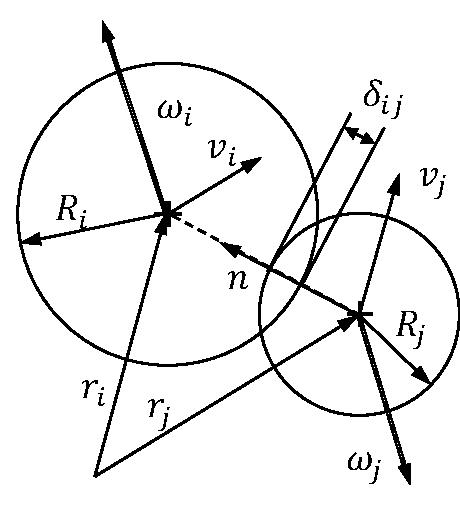
\includegraphics[scale=0.8]{collision.pdf}
  \centering
  \caption{Particle collision layout with the length of overlap $\delta$.}
  \label{fig:collision}
\end{figure}\vspace*{3pt}
The interaction force $F_i$ and torque $T_i$ in \equref{eq:restrictionDEM_EOM} can be determined using the collision model
\begin{flalign} \label{DEM_interactions}
&F_i=\sum_{j}{\left(F^n_{ij}+F^t_{ij}\right)} \\
&T_i=\sum_{j}{T_{ij}}
\end{flalign} itself
with $F_{ij}^n$ and $F_{ij}^t$ being the normal and tangential forces and $T_{ij}$ is the torque acting from particle $j$ to $i$.
\myparagraph{Normal contact force model}
The abovementioned overlapping length anneals the collision response of rigid objects by the $\delta$-dependent repulsive normal contact force model
\begin{flalign} \label{DEM_normal_force}
&F_{ij}^n=(k^n\delta+k^d v^n)n, \\
\end{flalign}
where $k^n$ and $k^d$ are the spring and damping coefficients of the collision, while $v^n=nv_{ji}$ is the normal component of the relative velocity $v_{ij}$.
\myparagraph{Tangential contact force and torque model}
The tangential or shear forces between colliding particles are determined by the relative linear and angular velocities $v_{ij}$ and $\omega_{ij}$. The tangential contact force model is written as
\begin{flalign} \label{DEM_tangential_force}
&F_{ij}^t=k^t v^t,
\end{flalign}
where 
\begin{flalign} \label{DEM_tangential_velocity}
&v^t=v_{ij}-(v_{ij}n)n+R_i'n\times\omega_i+R_j'n\times\omega_j,
\end{flalign}
is the relative tangential velocity denoting the actual distance of particle $i$ and the contact point with $R_i'=(R_i-\delta/2)$. Finally, the tangential contact forces are used to calculate the resultant torque of particle $i$:
\begin{flalign} \label{DEM_tangential_force}
&T_i=\sum_j{R_i'n\times F_{ij}^t}.
\end{flalign}
Note that particle interaction forces and torques are calculated only when $\delta>0$, otherwise, the particles $i$ and $j$ are not in interaction with each other. The equations \equref{eq:restrictionDEM_EOM} form a system of $N$ algebraic equations that can be solved explicitely.\\



\subsection{Temporal integration}
Numerical schemes for integration are required to solve time-dependent differential equations. Two numerical schemes are implemented in Nauticle.
\subsubsection{Explicit-Euler method}
This is a one-step explicit method to advance quantities in time by the
\begin{flalign}
\phi^{n+1}=\phi^n+\Delta t f(\phi^n,t^n)
\end{flalign}
expression, where $\phi$ is an arbitrary quantity, and $f(\phi^n,t^n)$ is a function of $\phi$ and time $t$ in the $n$th time instant, and $\Delta t=t^{n+1}-t^n$ is the time step size.
\subsubsection{Second-order Runge-Kutta method}
The second order explicit Runge-Kutta, or midpoint scheme consists of two integration steps. The first one is the prediction step
\begin{flalign}
\phi^{n+1/2}=\phi^n+\Delta t f(\phi^n,t^n),
\end{flalign}
which is followed by the evaluation of $f(\phi^{n+1/2},t^{n+1/2})$. The second step is the correction step to obtain the final value $\phi^{n+1}$, by using the intermediate step:
\begin{flalign}
\phi^{n+1}=\phi^n+\Delta t f(\phi^{n+1},t^{n+1}).
\end{flalign}


\section{Implementation}
\subsection{The Nauticle environment} \label{sec:environment}
The basic idea of the Nauticle environment is that any particle method (regardless of the classification in the previous section) can be considered as the determination of interactions between spatially distributed point-like nodes (particles). This assumption leads to the general interpretation of particle methods as \textit{interactions}. 

In this section the definitions corresponding to Nauticle are introduced, than the most important implementation methodologies and features of the solver are discussed.
\subsubsection{Definitions}
\textbf{Tensor}: Tensors in Nauticle have a few restrictions that are discussed here for the sake of clarity and simplicity. The tensor $T$ is a zeroth ($T\in\R$), first ($T\in\R^d$), or second ($T\in\R\otimes\R$) order real valued tensor, in $d=1,2,3$ dimensions. Throughout this guide tensors are considered to obey these restrictions, otherwise it is indicated.

\textbf{Domain}: Consider the simply connected rectangular subset $\Gamma^d\subset\R^d$ ($d=1,2,3$), with edge size $\lambda^d$ and its boundary $\partial\Gamma^d$. The $\Gamma^d$ subset is a $d$ dimensional domain, if the
\begin{flalign}
\begin{split}
&1.\quad \Gamma^d=[r_{min},r_{max}] \puretext{such that} r_{min}<r_{max} \puretext{and} \{r_{min},r_{max}\} \in \R^d\\
&2.\quad r \in \Gamma^d \puretext{if} r^d_{min}<r<r^d_{max} \\
&3.\quad \partial\Gamma^d=\bigcup_{d}{(r^d_{min}\cup r^d_{max})} \\
&4.\quad \lambda^d=r^d_{max}-r^d_{min}
\end{split}
\end{flalign}
conditions are satisfied.

\textbf{Particle}: A point-like object with position $r\in\Gamma^d$.

\textbf{Particle system}: The $P_{N}=\left\{r_i|i=1,2,...,N\right\}$ set of particles $r_i\in\Gamma^d$ is defined as a particle system of domain $\Gamma^d$.

\textbf{Field}: Consider a particle system $P_N$. The set $F_N=\left\{f_i\leftarrow P_N \vert i=1,2,...,N\right\}$ is a real valued zeroth, first or second order tensor field over $P_N$.

\textbf{Workspace}: A collection of user-defined constants, variables, fields and particle system representing the quantities of the physical model.

\textbf{User-defined equations (UDE)}: Expressions, built up using the workspace content. The evaluation of an equation means the assignment of the RHS solution to the LHS. Consequently the LHS should be a variable, field or particle system.

\subsection{n-nearest neighbour search} \label{sec:neighbour_search}
One of the specific properties of particle methods is the continually changing particle layout. Since no interparticle structure is considered, the connectivity may change (except for Lagrangian or unbounded mollifier) with the particle positions. The naive ($N^2$ complexity) determination of particle interactions is usually unsatisfactory due to its high performance requirement, therefore, a more efficient neighbour searching algorithm should be used instead. \\
To determine interparticle connectivity, the following steps are performed in Nauticle:
\begin{enumerate}
  \item Calculation of hash key for each particle using the unfolding the domain shown by Figure \ref{fig:unfolding},
  \item Sorting particles and the fields by the array of hash keys,
  \item Generating Start and End arrays containing the index of the first and last particle of each cell. The Start and End arrays are introduced in Figure \ref{fig:nnsearch}.
\end{enumerate}
Later, during the calculation of particle interactions, the adjacent cells of each particle are checked to find the potential neighbours. Finally, the actual neighbours are calculated based on the set of potential neighbours. Due to computational optimisation, the steps above are not performed until the particle layout is changed.

\begin{figure}[h]
  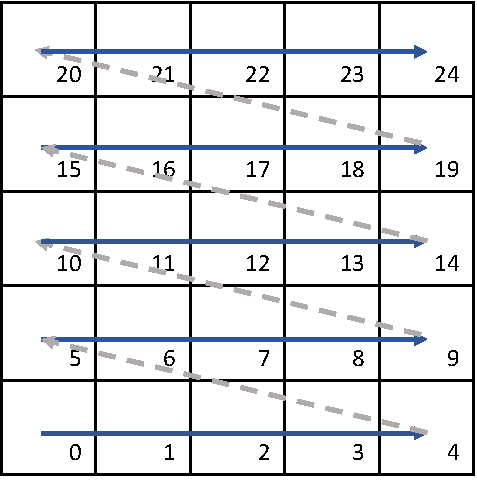
\includegraphics[scale=0.6]{hash_key.pdf}
  \centering
  \caption{Unfolding the two dimensional domain to one dimension. The same procedure can be applied in three dimensions.}
  \label{fig:unfolding}
\end{figure}\vspace*{3pt}
\begin{figure}[h!]
  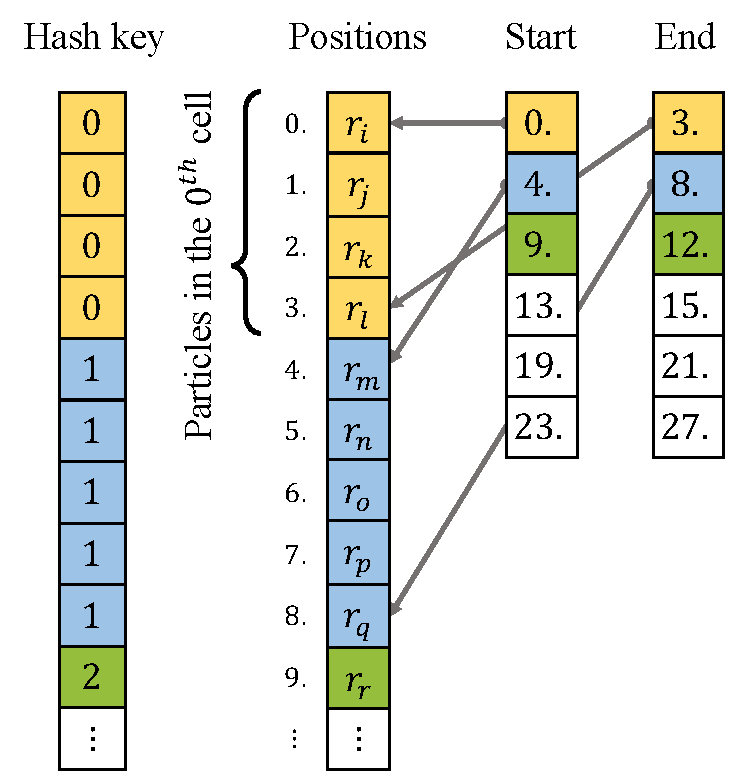
\includegraphics[scale=0.6]{nnsearch.pdf}
  \centering
  \caption{Indexing particle positions with Start and End arrays.}
  \label{fig:nnsearch}
\end{figure}\vspace*{3pt}
\subsection{Periodic and symmetric boundaries}
The computational domain $\Omega$ defined in (TODO) forms the particles' frame of reference. Since no particle can ever exist outside the domain, the bounding surface $\partial\Omega$ applies symmetric or periodic rules to avoid the exclusion by handling particles that intend to cross the surface. Obviously, the opposite boundaries of $\Omega$ have to be both symmetric or periodic boundaries.
Both conditions imply the repositioning of exiting particle $i$ applying the
\begin{flalign} \label{eq:restriction}
r_i\leftarrow r_i mod \lambda
\end{flalign}
restriction, where $\lambda$ is the size of $\Omega$. However, exiting should ideally never occur in case of symmetric boundary. The restriction \equref{eq:restriction} does not provide either correct periodic or symmetric boundary conditions in itself. To take these conditions into account, the overhanging influence radius should be replaced or reflected properly. The physical interpretation of influence radius in the vicinity of periodic ($\partial\Omega_p$) and symmetric ($\partial\Omega_s$) boundaries is shown in Figure \ref{fig:periodic_symmetric}.
\begin{figure}
  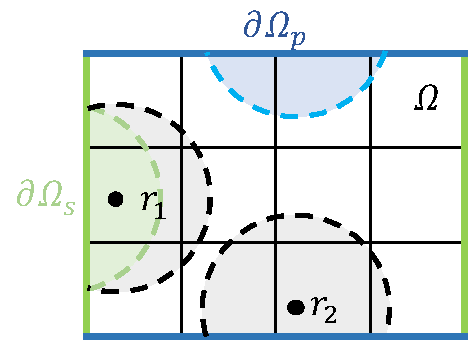
\includegraphics[scale=0.8]{periodic_symmetric_2.pdf}
  \centering
  \caption{ Shifting (blue) and reflecting (green) influence radius in the vicinity of periodic and symmetric boundary conditions respectively.}
  \label{fig:periodic_symmetric}
\end{figure}\vspace*{3pt}
During the calculation of interparticle distance at the boundary the ensemble formula
\begin{flalign} \label{eq:boundary_interparticle_distance}
&r_{ji}=r_{ji}+\beta\delta(\delta-1)(r_{max}-r_j)+\beta\delta(\delta+1)(r_{min}-r_j)+(\beta-1)\floor{\frac{r_{ji}-r_{min}}{\lambda}}\lambda
\end{flalign}
is applied, where $\beta=0$ or $1$ for periodic or symmetric boundaries respectively, $\lambda$ is the size of $\Omega$, the operator $\floor{\cdot}$ denotes floor, and
\begin{flalign} \label{eq:delta_perioic_symmetric}
&\delta=-\floor{\frac{g_j-r_{min}}{N_c}},
\end{flalign}
with $g_j$ being the grid coordinate of particle $j$ and $N_c$ denotes the number of cells along $\Omega$. The grid coordinates of the adjacent particles is calculated by
\begin{flalign} \label{eq:grid_position_periodic_symmetric}
&g_j\leftarrow g_j+\delta(N_c-\beta N_c+\beta).
\end{flalign}
Since in case of the symmetric condition the interactions calculated by particle mirroring, the vector and tensor quantities should be reflected using the reflection matrix
\begin{flalign} \label{eq:reflection_periodic_symmetric}
&R=\sum_{i=1}^d{I_{ii}(-2\beta_i+1)},
\end{flalign}
where $I$ is a $d$ dimensional identity tensor. Note that in one dimension ($d=1$), it is required to distinguish scalars and single element vectors, because scalar quantities should remain the same after reflection.



\subsection{Expression tree}
The generality of the numerical model requires the analysis of user-defined expressions and equations (see Section \ref{UDE}). In Nauticle the expression parsing is based on the expression tree shown in Figure \ref{fig:expression_tree}.
\begin{figure}[h!]
  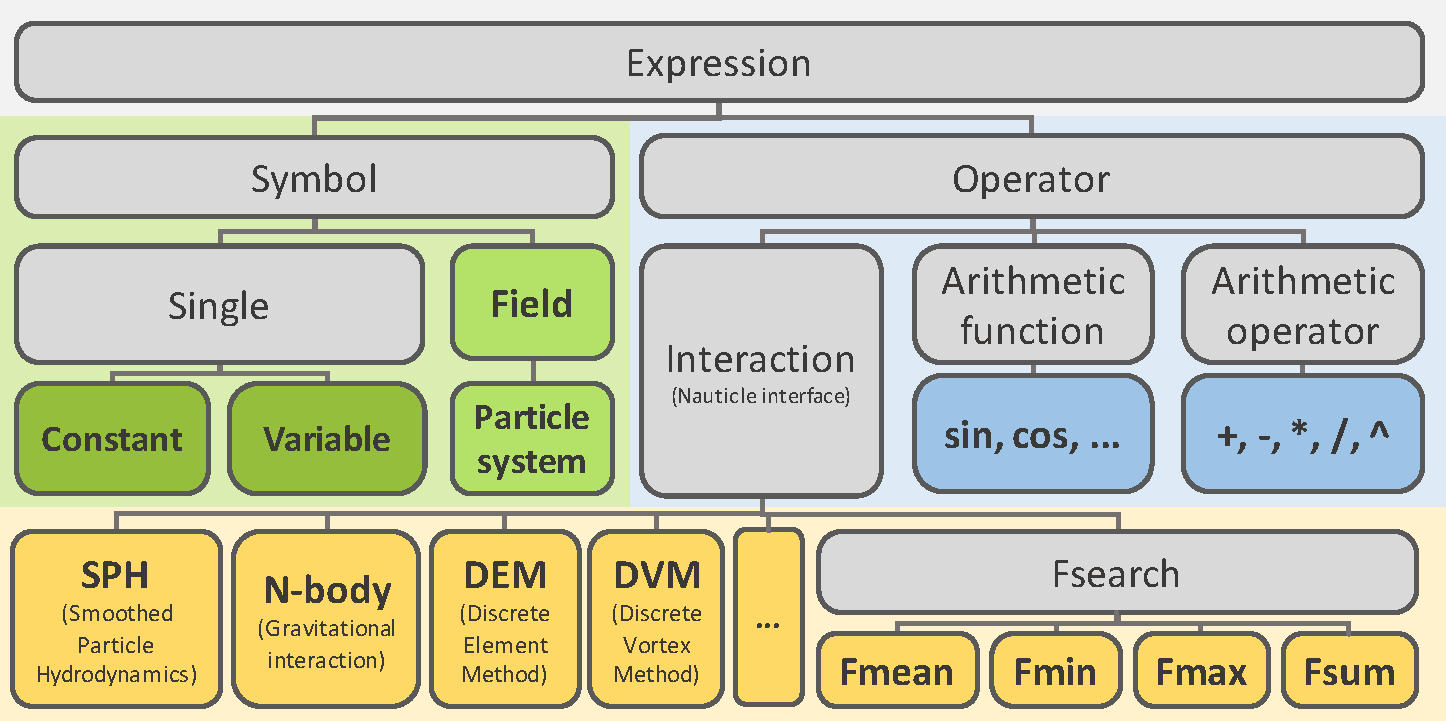
\includegraphics[scale=0.5]{expression_tree.pdf}
  \centering
  \caption{Expression tree: hierarchy of expression elements. The gray nodes in the tree indicate abstract types.}
  \label{fig:expression_tree}
\end{figure}\vspace*{3pt}

Using the nodes of the expression tree the user-defined expressions can be constructed and solved recursively. A simple example is presented by the Figure \ref{fig:expression_example}.
\begin{figure}[h]
  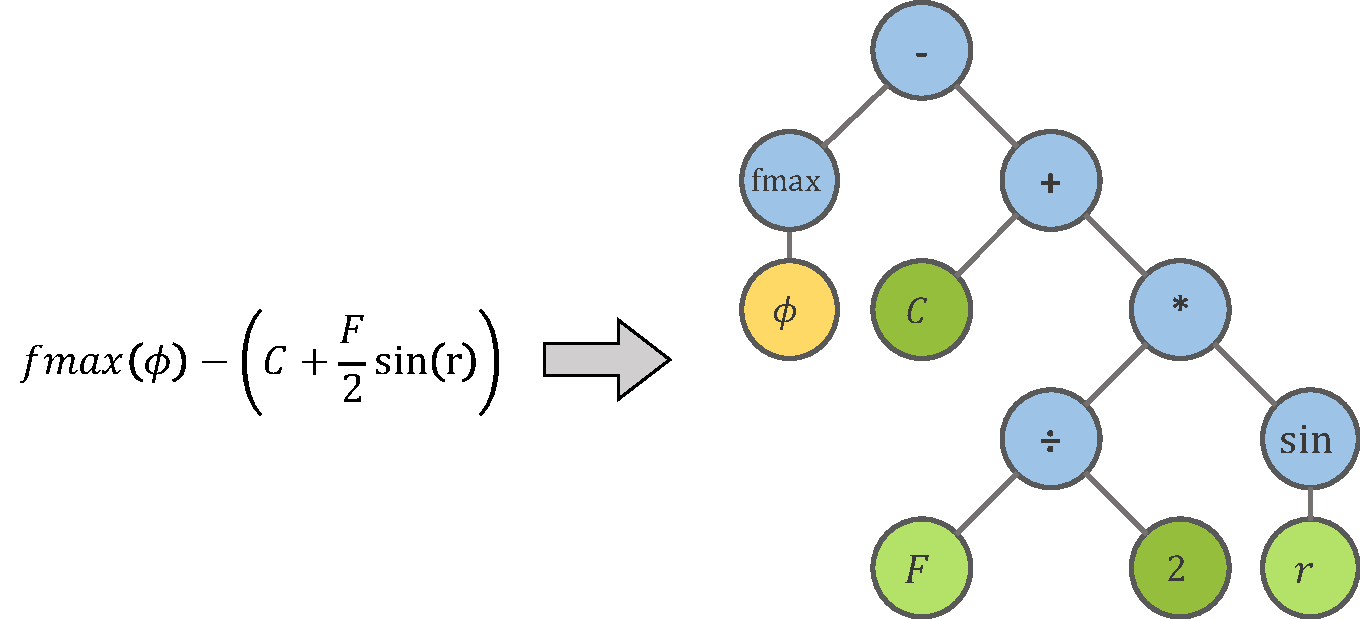
\includegraphics[scale=0.5]{expression_example.pdf}
  \centering
  \caption{Example for construction of expressions using the nodes of the expression tree.}
  \label{fig:expression_example}
\end{figure}\vspace*{3pt}

Although the nodes of the expression tree implements different quantities and operators of Nauticle, all nodes are considered as tensors. In the following, the branches and nodes of the expression tree is discussed.

\subsubsection{The term branch}
On the one hand, the single terms like constants and variables represent global values for the simulation such as time step size or gravity, which usually have the same value for each particle, consequently one (single) instance is sufficient to be stored. Therefore the single quantities have very small memory requirement. However, in case of multistep integrators, the desired number of former values of variables are automatically stored. Obviously it is unnecessary for the constant values, since their values cannot be changed during their lifetime. On the other hand, the fields are interpreted over a set of spatial nodes (particles) storing tensor values assigned for each of the particles. Former values for multistep integrators are automatically stored as well as in case of the variables. A special implementation of a field is the particle system itself, storing the particle positions as field variables. The particle system is special not only because of storing particle positions but it performs n-nearest neighour search and stores the computational domain too. The restriction of particles to the domain is also performed by the particle system.

\subsubsection{The operator branch}
The other main branch of the expression tree is the branch of operators acting on terms. Operators are classified into three groups:
\begin{itemize}
  \item Arithmetic operators,
  \item Arithmetic functions,
  \item Interactions.
\end{itemize}
The first two groups of operators evaluate operations on single quantities or particlewise field quantities (e.g. addition of two fields), while the interactions deal operations require field data (e.g. value of field maximum or minimum).
\myparagraph{Arithmetic operators}
The supported arithmetic operators are presented in Table \ref{tbl:arop}.
\begin{table}
\begin{center}
\caption{Supported arithmetic operators in Nauticle.}\label{tbl:arop}
\begin{tabular}{ l c c c c }
\toprule[1.5pt]
\bf Operator name & \bf Sign & \bf Operands & \bf Description\\ 
\midrule
Addition & "+" & 2 & $[n \times m] + [n \times m]$\\ 
Subtraction & "-" & 2 & $[n \times m] - [n \times m]$\\ 
Product & "*" & 2 & $[n \times m] * [m \times n]$\\ 
Term by term product & ":" & 2 & $[n \times m] : [n \times m]$\\ 
Power & "$\hat{\ }$" & 2 & $[n \times m] \hat{\ } [1 \times 1]$\\ 
Positive & "+" & 1 & $[n \times m]$\\ 
Negative & "-" & 1 & $[n \times m]$\\ 
\bottomrule[1.25pt]
\end{tabular}
\end{center}
\end{table}
The arithmetic operators are valid for tensors with sizes that are in agreement (last column of Table \ref{tbl:arop}).
\myparagraph{Arithmetic functions}
The arithmetic functions supported by Nauticle are summarised in Table \ref{tbl:arfc}. It should be noted here that complex numbers are currently not supported by the tensor implementation, therefore some of the functions may give uninterpretable results (e.g. $\sqrt{-1}$ is not a number in Nauticle).
\begin{table}
\begin{center}
\caption{Supported arithmetic functions in Nauticle.}\label{tbl:arfc}
\begin{tabular}{ l l c | l l c }
\toprule[1.5pt]
\bf Funcion & \bf Name & \bf Op's & \bf Funcion & \bf Name & \bf Op's\\ 
\midrule
Absolute value & $abs$ & 1 & Modulo & $mod$ & 2 \\
Arc cosine & $acos$ & 1 & Random in range & $rand$ & 2 \\
Arc co-tangent & $acot$ & 1 & Sign & $sgn$ & 1 \\
Arc sine & $asin$ & 1 & Sine & $sin$ & 1 \\
Arc tangent & $atan$ & 1 & Sine hyperbolic & $sinh$ & 1 \\
Cosine & $cos$ & 1 & Square root & $sqrt$ & 1 \\
Cosine hyperbolic & $cosh$ & 1 & Tangent & $tan$ & 1 \\
Co-tangent & $cot$ & 1 & Tangent hyperbolic & $tanh$ & 1 \\
Co-tangent hyperbolic & $coth$ & 1 & Trace & $trace$ & 1 \\
Cross product & $cross$ & 2 & Tanspose & $transpose$ & 1 \\
Exponential & $exp$ & 1 & Trunc & $trunc$ & 1 \\
Floor & $floor$ & 1 & Matrix determinant & $determinant$ & 1 \\
Greater than & $gt$ & 2 & Matrix inverse & $inverse$ & 1 \\
Natural logarithm & $log$ & 1 & Equal & $eq$ & 2 \\
Less than & $lt$ & 2 & Boolean and & $and$ & 2 \\
Vector lenght & $magnitude$ & 1 & Boolean or & $or$ & 2 \\
Maximum & $max$ & 2 & Boolean negation & $not$ & 1 \\
Minimum & $min$ & 2 & Boolean exclusive or & $xor$ & 2 \\
Tensor element & $elem$ & 3 & Boolean condition & $if$ & 3 \\
\bottomrule[1.25pt]
\end{tabular}
\end{center}
\end{table}

\myparagraph{Interactions}
It was pointed out earlier in Section \ref{sec:environment} that any particle method can be considered as a collection of particle interaction laws. Due to that, the interaction branch forms an essential part of not only the expression tree but even the Nauticle environment. This group of operators deals with particle interactions that certainly depend on field quantities (and particle system). Furthermore the interaction branch provides an intermediate development interface, which is introduced in detail later in Section \ref{sec:interface}.
The simplest functions in this branch are presented in Table \ref{tbl:fsearch}. Since the magnitude of arbitrary tensor quantities is ambiguous, these field-functions can be evaluated only over scalar fields (last column of Table \ref{tbl:fsearch}). These functions have linear computational complexity.
\begin{table}
\begin{center}
\caption{Simple interaction operators.}\label{tbl:fsearch}
\begin{tabular}{ l l c c }
\toprule[1.5pt]
\bf Operator & \bf Name & \bf Operands & \bf Description\\
\midrule
Field maximum & $fmax$ & 1 & $[1 \times 1]$\\ 
Field minimum & $fmin$ & 1 & $[1 \times 1]$\\ 
Field average & $fmean$ & 1 & $[1 \times 1]$\\
\bottomrule[1.25pt]
\end{tabular}
\end{center}
\end{table}
More complicated operators in Nauticle belong to the particle methods presented in Section \ref{sec:implemented}.


\section{Using Nauticle}
\subsection{Simulation workflow} \label{sec:sim_workflow}
% \subsection{Solver}
% To define a simulation case you need to create a form to pass to the solver. The form contains all the required information about the physical model including a workspace and the list of equations. In this section the structure of the form is discussed through the introduction of the workspace and the user-defined equations.
% \subsubsection{Workspace}
% Workspace is a fundamental part of the solver. The workspace contains all the constants, variables, fields and the particle system. 
% \subsubsection{User-defined equations} \label{UDE}
% \subsection{Parameter space}
\subsection{Input/Output file formats}
During a simulation execution, Nauticle works with four types of input and output files. Some of these files are fundamental, the others are optional. The subsequent sections introduce these files more or less in the order of proirity.
\subsubsection{VTK-document}
\subsubsection{XML-document}
The XML-document is the most important and fundamental input file of any simulation executed by Nauticle. The XML-documents are distinguished by the data they carry. A minimal document is presented in Figure \ref{fig:xml_intro}.
\begin{figure}[h!]
  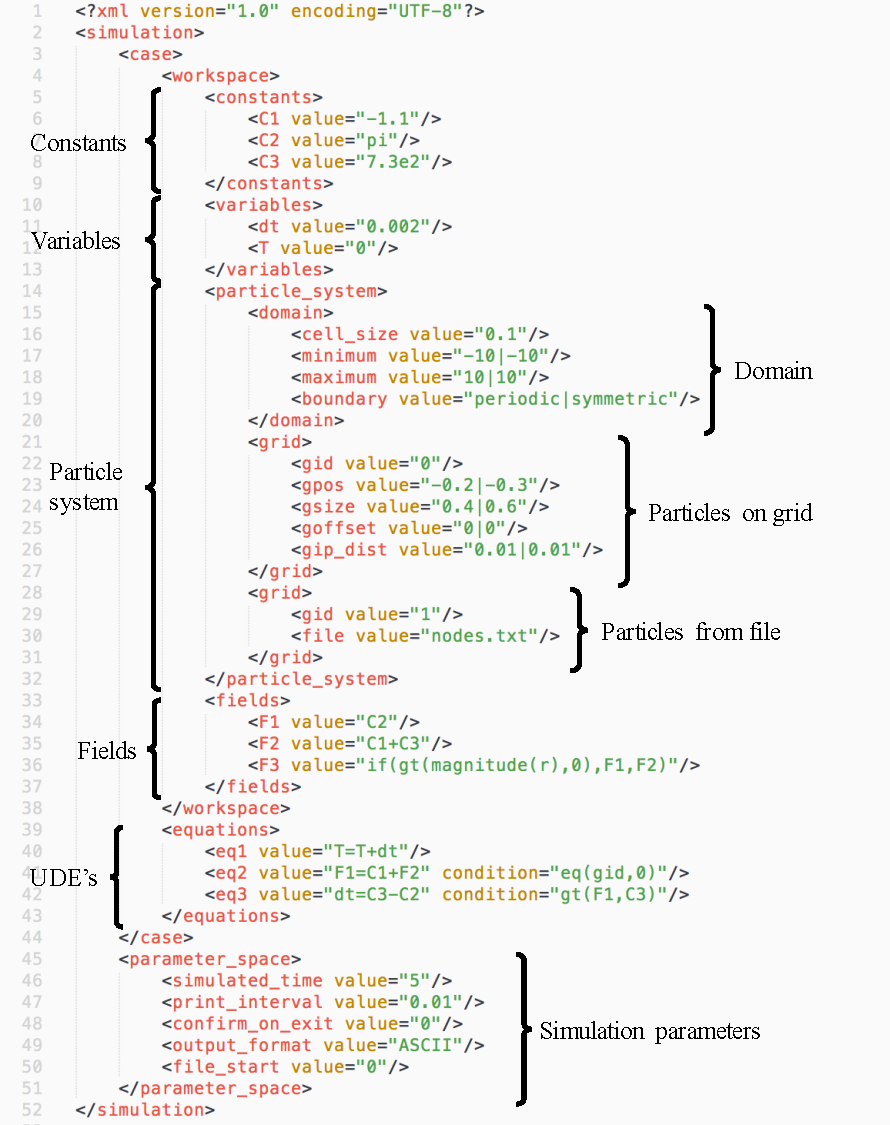
\includegraphics[scale=1]{xml_intro.pdf}
  \centering
  \caption{Structure of the XML-document.}
  \label{fig:xml_intro}
\end{figure}\vspace*{3pt}
Using the document of Figure \ref{fig:xml_intro} the whole workspace and list of equations to be passed to the solver are defined and no external sources are used except for the nodal coordinates. Another way of problem initialisation is the application of a former simulation result stored in VTK file. Despite of that, XML-documents cannot be ommitted, but they are used to refer to the desired input file. This type of initialisation allows a significantly simpler XML-document as it is illistrated in Figure \ref{fig:xml_intro_simple}.
\begin{figure}[h!]
  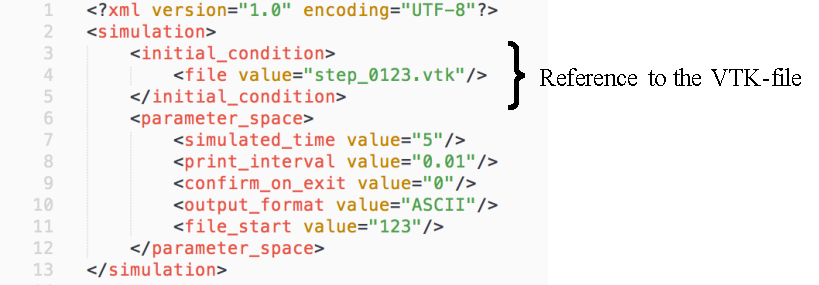
\includegraphics[scale=1]{xml_intro_simple.pdf}
  \centering
  \caption{Structure of the XML-document refer to the former simulation result.}
  \label{fig:xml_intro_simple}
\end{figure}\vspace*{3pt}
Note that in this configuration the workspace and list of equations are also stored in the VTK-document.
\subsubsection{Text document}
The particle layout can be optionally defined through text files containing the set of nodal positions instead of the uniform grid generation based on the XML data. Note that the text file should always contain three dimensional coordinates separated by spaces or tabs. The dimensions of the problem is then defined by the domain and only the relevant coordinates of the nodal positions are considered, other coordinates are dropped.
\subsubsection{Logging}
The simulation log file contains the simulation data as it appears in terminal during runtime. Each execution produces a single log file with the name "sim.log" by default. A previous log file with the same name in the working directory is purged at the beginning of the calculation without approval.
% vtk, xml, log, xyz
\subsection{Runtime commands}
There are further optional commands that cannot be defined in the XML-document. These are the runtime commands summarised in Table \ref{tbl:runtime_commands}. To obtain information about the reserved names you need to use the "-wsres" command. Nauticle offers parallelisation on multicore CPU systems. By default, the number of threads to use during the execution is the number of available threads. Hovewer, you may want to limit the solver by defining the actual number threads to use. This can be done by the "-numthreads N" command, where N is the desired number of threads. 
\begin{table} [h]
\begin{center}
\caption{Runtime commands.} \label{tbl:runtime_commands}
\begin{tabular}{ l l l }
\toprule[1.5pt]
\bf  & \bf Command & \bf Description\\
\midrule
1. & -help & Display Nauticle information. \\
2. & -wsres & Lists all reserved names in workspace. \\
3. & -numthreads <number> & Defines the number of threads to use. Default is detected. \\
4. & -xmlname <filename> & Defines the name of the XML input file. \\
5. & -logfile <filename> & Defines the name of the output log file. \\
6. & -wdir <directory> & Defines the working directory. Full path is required. \\
7. & -version & Prints the version number. \\
\bottomrule[1.25pt]
\end{tabular}
\end{center}
\end{table}

\section{Installation}
\subsection{Requirements}
Please note that currently, the installation process does not support Windows, it works only on Linux (distributions that support Application Package Tool (APT)) and Mac OSX systems.  Hereinafter Linux is considered to support APT.
Nauticle requires a few dependencies and requirements to be installed. These are the following:
\begin{itemize}
  \item cmake (at least version 3.5) (\myhref{https://cmake.org/download/}{https://cmake.org/download/}),
  \item Visualization Toolkit 7.0.0 (\myhref{http://www.vtk.org/files/release/7.0/VTK-7.0.0.zip}{http://www.vtk.org/files/release/7.0/VTK-7.0.0.zip}),
  \item Common utilities (TODO),
  \item ProLog (TODO),
  \item HandyXML (TODO).
\end{itemize} 
Details of the required dependencies are not discussed here, please follow the links to find more information about the listed software. Further dependencies could be required by the Visualization Toolkit.

During the installation process it is assumed that the user has internet connection and root privileges in the operating system. Throughout the following two subsections the manual and automatic installation procedures are discussed in detail.
Note: to avoid any version conflicts it could be preferable to install and build Nauticle and its dependencies using HashDist, which is an environment management system (\myhref{https://github.com/hashdist/hashdist}{https://github.com/hashdist/ hashdist}). However it is not mandatory and the automated installation process does not apply HashDist.
\subsection{Automated installation}
Although it is possible to install and build the dependencies and Nauticle manually, it is recommended to use the installation shell script arrives with Nauticle. The script installs the whole package including the dependencies by typing the command
\begin{lstlisting}[language=bash]
  $ sh (*@\installer{}@*)
\end{lstlisting}
in terminal after changing direcotry to the desired folder. The content of the script with explanations is as follows:

\begin{example}{\installer{}}{}
\lstset{basicstyle=\tiny}
\begin{lstlisting}[language=bash]
  #!/bin/sh

  # Set current directory to install directory.
  INSTALL_DIR=$PWD
  sudo chmod -R 777 ${INSTALL_DIR}

  # Set OS variable (assume linux)
  OS="Linux"
  if [ "$(uname)" = "Darwin" ]; then
  # if mac, install wget, and cmake
      brew install wget
      brew install cmake
      OS="Mac"
  elif [ $OS = "Linux" ]; then
  # if linux, install opengl and cmake
    sudo apt-get update
    sudo apt-get --yes --force-yes install build-essential
    sudo apt-get --yes --force-yes install freeglut3-dev
    sudo apt-get --yes --force-yes install cmake
  fi

  # Install proper version of VTK library
  wget http://www.vtk.org/files/release/7.0/VTK-7.0.0.zip
  sudo unzip VTK-7.0.0.zip -d /usr/local/
  cd /usr/local/VTK-7.0.0
  sudo cmake .
  sudo make

  # Go to install directory
  cd $INSTALL_DIR

  # Download and unzip the required packages
  # Common utils
  wget https://bitbucket.org/Nauticleproject/commonutils/downloads/commonutils-1.0.170221.zip
  sudo unzip commonutils-1.0.170221.zip
  sudo chmod -R 777 commonutils
  rm commonutils-1.0.170221.zip
  # Prolog
  wget https://bitbucket.org/Nauticleproject/prolog/downloads/prolog-1.0.170221.zip
  sudo unzip prolog-1.0.170221.zip
  sudo chmod -R 777 prolog
  rm prolog-1.0.170221.zip
  # HandyXML
  wget https://bitbucket.org/Nauticleproject/handyxml/downloads/handyxml-1.0.170221.zip
  sudo unzip handyxml-1.0.170221.zip
  sudo chmod -R 777 handyxml
  rm handyxml-1.0.170221.zip
  # Nauticle
  wget https://bitbucket.org/Nauticleproject/Nauticle/downloads/Nauticle-1.0.170221.zip
  sudo unzip Nauticle-1.0.170221.zip
  sudo chmod -R 777 Nauticle
  rm Nauticle-1.0.170221.zip

  # Install the dependencies and the Nauticle executable (pmsimple) itself
  cd commonutils
  sudo cmake .
  sudo cmake .
  sudo make install
  cd ..
   
  cd prolog
  sudo cmake .
  sudo cmake .
  sudo make install
  cd ..
   
  cd handyxml
  sudo cmake .
  sudo cmake .
  sudo make install
  cd ..

  # Set sirectory name for executable
  BIN_DIR="${INSTALL_DIR}/Nauticle/bin/$OS"
  cd Nauticle
  sudo cmake .
  sudo cmake .
  sudo mkdir $BIN_DIR
  sudo make
  cd ..

  # Add pmsimple to the environmental PATH variable
  if [ "$OS" = "Mac" ]; then
    sudo printf "\nexport PATH=\${PATH}:$BIN_DIR\n" >> ~/.bash_profile
      alias brc='source ~/.bashrc'
  elif [ "$OS" = "Linux" ]; then
    sudo printf "\nexport PATH=\${PATH}:$BIN_DIR\n" >> ~/.bashrc
    alias brc='source ~/.bashrc'
  fi

  # Generate optional script file to run pmsimple 
  sudo rm -f start.sh
  sudo touch start.sh
  sudo chmod 777 start.sh
  printf "#!/bin/sh\nexecutable=$BIN_DIR/pmsimple\n" >> start.sh
  printf "sudo \$executable" >> start.sh
\end{lstlisting}
\end{example}

It downloads and builds the necessary files in your system. After installation, the executable (\execname{}) will be placed in the bin directory and a \textbf{start.sh} file will be generated in the installation directory. The installer also adds the bin directory to your environment variables so you can run it from different directories. To activate this feature it could be necessary to manually reload the \textbf{.bash\_profile} or \textbf{.bashrc} file in your home directory using the \texttt{source} command.
In certain cases, when environment variables are not available you can perform computations using the \textbf{start.sh} file in the simulation folder:
\begin{lstlisting}[language=bash]
  $ sh start.sh
\end{lstlisting}
Note that running Nauticle with the generated \textbf{start.sh} file does not allow to pass arguments to the solver in terminal. Any options should be placed in the \textbf{start.sh} file instead.


\section{Nauticle interface} \label{sec:interface}
\section{The Nauticle open-source code}
This section comments the role of each source and header file of Nauticle. For better clarity the explanation is divided into different groups marked by the subsequent sections.
\subsection{Nodes of the expression tree}
\subsubsection{Particlewise nodes}
\textbf{pmExpression.h / pmExpression.cpp} \\
Declares / defines the expression node of the expression tree. This is an abstract class. \\

\textbf{pmTerm.h / pmTerm.cpp} \\
Declares / defines the term node of the expression tree. This is an abstract class. \\

\textbf{pmSingle.h / pmSingle.cpp} \\
Declares / defines the single node of the expression tree. This is an abstract class. \\

\textbf{pmConstant.h / pmConstant.cpp} \\
Declares / defines the node for constants in the expression tree. \\

\textbf{pmVariable.h / pmVariable.cpp} \\
Declares / defines the node for variables in the expression tree. \\

\textbf{pmField.h / pmField.cpp} \\
Declares / defines the field node of the expression tree. \\

\textbf{pmParticle\_system.h / pmParticle\_system.cpp} \\
Declares / defines the particle system node of the expression tree. It performs neighbour searching. \\

\textbf{pmArithmetic\_function.h} \\
Declares / defines the node for arithmetic functions in the expression tree. \\

\textbf{pmArithmetic\_operator.h} \\
Declares / defines the node for arithmetic operators in the expression tree. \\


\subsubsection{Nodes for interaction branch}
\textbf{pmInteraction.h} \\
Declares / defines the interaction node in the expression tree. This is an abstract class. It manages the interparticle connections. \\

\textbf{pmFsearch.h / pmFsearch.cpp} \\
Declares / defines the class for field search algorithms. This is an abstract class. \\

\textbf{pmFmin.h / pmFmin.cpp} \\
Declares / defines the functions for minimum search of a field.  \\

\textbf{pmFmax.h / pmFmax.cpp} \\
Declares / defines the functions for maximum search of a field. \\

\textbf{pmFmean.h / pmFmean.cpp} \\
Declares / defines the functions for mean calculation of a field. \\

\textbf{pmNbody.h / pmNbody.cpp} \\
Declares / defines the functions for particle interactions. It calculates the gravitational forces. \\

\textbf{pmNeighbours.h / pmNeighbours.cpp} \\
Declares / defines the functions for particle interactions. It calculates the number of neighbours in a given distance. \\

\textbf{pmDem.h} \\
Declares / defines the node in the expression tree to calculate interactions based on Discrete Element Method (DEM). \\

\textbf{pmOperator.h} \\
Declares / defines the operator node in the expression tree. This is an abstract class. \\

\textbf{pmSph.h} \\
Declares / defines the Smoothed Particle Hydrodynamics (SPH) node in the expression tree. This is an abstract class. \\

\textbf{pmSph\_operator.h} \\
Declares / defines functions for SPH interactions and differential operators. \\

\subsubsection{Files for simulation case}

\textbf{pmCommand\_parser.h / pmCommand\_parser.cpp} \\
Declares / defines the functions that manage terminal commands. \\

\textbf{pmTensor.h / pmTensor.cpp} \\
Declares / defines the class that implements functions for tensor quantities. \\

\textbf{pmTensor\_parser.h / pmTensor\_parser.cpp} \\
Declares / defines the functions that analyse tensors based on expressions. \\

\textbf{pmParameter\_space.h / pmParameter\_space.cpp} \\
Declares / defines the functions for parameter management. \\

\textbf{pmCase.h / pmCase.cpp} \\
Declares / defines the functions that read the configuration file, build and run the simulation through the solver. \\

\textbf{pmDomain.h / pmDomain.cpp} \\
Declares / defines the rectangular simulation domain class in which the particles exist. \\

\textbf{pmMath\_parser.h / pmMath\_parser.cpp} \\
Declares / defines the functions for string parsing. \\

\textbf{pmMath\_test.h / pmMath\_test.cpp} \\
Declares / defines the class that performs mathematical expressions stored in string format. This is an abstract class. \\

\textbf{pmExpression\_parser.h / pmExpression\_parser.cpp} \\
Declares / defines the functions for expression parsing. \\

\textbf{pmEquation\_parser.h / pmEquation\_parser.cpp} \\
Declares / defines the class that analyses user defined equations of the configuration file. \\

\textbf{pmEquation.h / pmEquation.cpp} \\
Declares / defines the class for user defined equations. It contains two expressions (LHS and RHS). It performs the evaluation too. \\

\textbf{pmWorkspace.h / pmWorkspace.cpp} \\
Declares / defines the class that manages user defined variables, constants, fields, and particle system. \\

\textbf{pmSolver.h / pmSolver.cpp} \\
Declares / defines the class that manages workspace and user defined equations. It solves the equations too. \\

\textbf{pmGrid.h / pmGrid.cpp} \\
Declares / defines the class for particle generation. Two ways: rectangular grid, or particles from .xyz file. \\

\textbf{pmGrid\_space.h / pmGrid\_space.cpp} \\
Declares / defines the class that manages, merges grids. \\

\textbf{pmVTK\_manager.h / pmVTK\_manager.cpp} \\
Declares / defines the functions for VTK reading and writing. This is an abstract class. \\

\textbf{pmVTK\_reader.h / pmVTK\_reader.cpp} \\
Declares / defines the functions for VTK reading. \\

\textbf{pmVTK\_writer.h / pmVTK\_writer.cpp} \\
Declares / defines the functions for VTK writing. \\

\textbf{pmXML\_processor.h / pmXML\_processor.cpp} \\
Declares / defines the functions for extracting data from xml file. \\

\subsubsection{Other files}
\textbf{pmRandom.h / pmRandom.cpp} \\
Declares / defines the functions for random number generation in a range. \\

\textbf{pmLog\_stream.h / pmLog\_stream.cpp} \\
Declares / defines the class that manages logging into file and terminal. \\

\textbf{pmSort.h}\\
Implements functions for sorting and reordering.\\

\textbf{pmKernel.h / pmKernel.cpp} \\
Declares / defines the functions for SPH kernels.\\

\textbf{pm.h}\\
Wraps includes.\\

\textbf{pmNoncopyable.h}\\
Implements a class for objects that are not allowed to be copied.\\

\textbf{pmVersion.h}\\
Contains Nauticle version information.\\




\section{Licenses}
\subsection{VTK license}
VTK is an open-source toolkit licensed under the BSD license.\\
Copyright (c) 1993-2008 Ken Martin, Will Schroeder, Bill Lorensen \\
All rights reserved.\\
Redistribution and use in source and binary forms, with or without modification, are permitted provided that the following conditions are met: \\
- Redistributions of source code must retain the above copyright notice, this list of conditions and the following disclaimer. \\
- Redistributions in binary form must reproduce the above copyright notice, this list of conditions and the following disclaimer in the documentation and/or other materials provided with the distribution. \\
- Neither name of Ken Martin, Will Schroeder, or Bill Lorensen nor the names of any contributors may be used to endorse or promote products derived from this software without specific prior written permission.\\

THIS SOFTWARE IS PROVIDED BY THE COPYRIGHT HOLDERS AND CONTRIBUTORS “AS IS” AND ANY EXPRESS OR IMPLIED WARRANTIES, INCLUDING, BUT NOT LIMITED TO, THE IMPLIED WARRANTIES OF MERCHANTABILITY AND FITNESS FOR A PARTICULAR PURPOSE ARE DISCLAIMED. IN NO EVENT SHALL THE AUTHORS OR CONTRIBUTORS BE LIABLE FOR ANY DIRECT, INDIRECT, INCIDENTAL, SPECIAL, EXEMPLARY, OR CONSEQUENTIAL DAMAGES (INCLUDING, BUT NOT LIMITED TO, PROCUREMENT OF SUBSTITUTE GOODS OR SERVICES; LOSS OF USE, DATA, OR PROFITS; OR BUSINESS INTERRUPTION) HOWEVER CAUSED AND ON ANY THEORY OF LIABILITY, WHETHER IN CONTRACT, STRICT LIABILITY, OR TORT (INCLUDING NEGLIGENCE OR OTHERWISE) ARISING IN ANY WAY OUT OF THE USE OF THIS SOFTWARE, EVEN IF ADVISED OF THE POSSIBILITY OF SUCH DAMAGE.

\subsection{Nauticle}
\noindent
Copyright \textcopyright{} 2017 by Balazs Toth \\
\noindent
BME Budapest University of Technology and Ecnonimcs, Department of Hydraulic and Water Resources Engineering\\

Nauticle is free software: you can redistribute it and/or modify it under the terms of the GNU Lesser General Public License as published by the Free Software Foundation, either version 3 of the License, or (at your option) any later version Nauticle is distributed in the hope that it will be useful, but WITHOUT ANY WARRANTY; without even the implied warranty of MERCHANTABILITY or FITNESS FOR A PARTICULAR PURPOSE.  See the GNU Lesser General Public License for more details You should have received a copy of the GNU Lesser General Public License along with Nauticle.  If not, see \myhref{http://www.gnu.org/licenses/}{http://www.gnu.org/licenses/}\\
 For more information please visit: \myhref{https://bitbucket.org/Nauticleproject/}{https://bitbucket.org/Nauticleproject/}


\end{document}